\lecture[2022-05-21]{Pandas II: Grouping, Aggregation, Pivot Tables Merging}

\subsection{Adding, Modifying, and Removing Columns}
Previously, we saw how we could find the most popular male names in California using \mintinline{text}{query} and sorting the result.

\begin{minted}{python}
babynames.query("Sex ==M and Year == 2020").sort_values("Count", ascending=False) # chooses only rows from 2020 which are male, then sort in descending order
\end{minted}

\begin{figure}[ht]
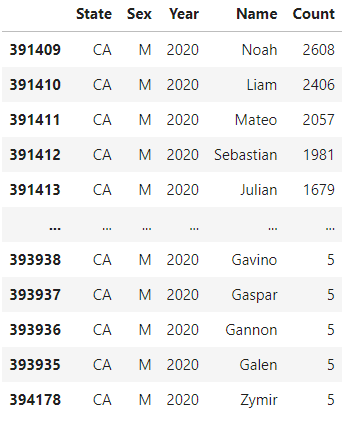
\includegraphics[width=0.4\textwidth]{4-sort1.png}\centering
\end{figure}

However, how can we find the longest names? If we sort by the names column, it will just return the names in reverse alphabetical order. After some searching, it turns out you can add in a \mintinline{text}{key} parameter which tells Pandas how to sort the values in the column.

\begin{minted}{python}
# start process - sorts names by alphabetical order
babynames.query("Sex == M and Year == 2020").sort_values("Name", ascending=False)
# new code - add key of baby name length
babynames.query("Sex == M and Year == 2020").sort_values("Name", key=lambda name: name.str.len(), ascending=False)
\end{minted}

\begin{figure}[ht]
\begin{minipage}{0.5\textwidth}
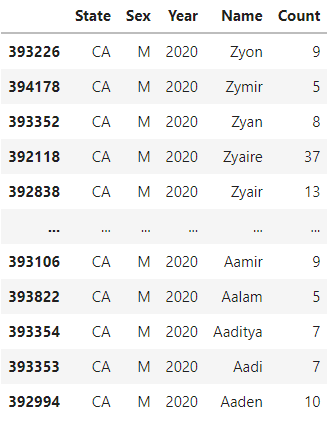
\includegraphics[width=0.65\textwidth]{4-sort2.png}\centering
\end{minipage}
\begin{minipage}{0.5\textwidth}
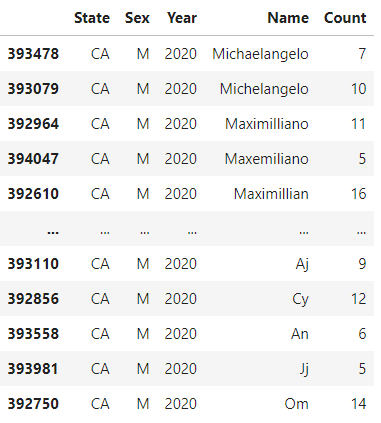
\includegraphics[width=0.65\textwidth]{4-sort3.png}\centering
\end{minipage}
\caption{The first approach only yields the names in reverse alphabetical order, but sorting with the \mintinline{text}{key} parameter yields the desired result.}
\end{figure}

However, this wasn't a feature until 2020. Prior to that, we would need to come up with another solution: 
\begin{itemize}
\item Create a temporary column getting the length of the baby name.
\begin{itemize}
\item Create a new series with only lengths.
\item Add the series to the dataframe.
\end{itemize}
\item Sort using that column.
\item Drop the temporary column. (General Form: \mintinline{text}{df.drop(<name>, (axis="columns"))})
\end{itemize}

\begin{minted}{python}
# creating a new column 
babynames["name_lengths"] = babynames["Name"].str.len() # new series - applies len to the Name series, then assigns the series "name_lengths" to the dataframe as a column
babynames = babynames.sort("name_lengths", ascending=False) # sort by name_length columns in descending order
babynames = babynames.drop("name_lengths", axis="columns") # drop the column - add axis = "columns" to specify it is a column (default drop rows)
\end{minted}

\subsubsection{Sorting by Arbitrary Functions}
To sort by arbitrary functions (e.g. \# occurrences of ``dr'' and ``ea'' in a string), use \mintinline{text}{Series.map} method. (Think of the \mintinline{text}{tbl.apply()} method in datascience)

\begin{minted}{python}
def dr_ea_count(string):
    return string.count("dr") + string.count("ea")

babynames["dr_ea_count"] = babynames["Name"].map(dr_ea_count) # Series.map(<func>)
babynames.sort_values("dr_ea_count", ascending=False)
\end{minted}
\begin{figure}[ht]
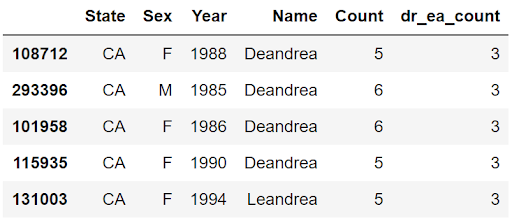
\includegraphics[width=0.5\textwidth]{4-map.png}\centering
\end{figure}

\subsection{Group By}
Let's try to find the female baby name whose popularity has fallen the most using RTP (ratio to peak - current number over peak number in a year).

e.g. for the name ``Jennifer'' measured in 2020, there were 172 Jennifers over the peak of 6064 Jennifers in 1972. Therefore, the RTP is $\frac{172}{6064} = 0.0233$.
\begin{figure}[ht]
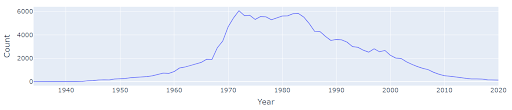
\includegraphics[width=0.75\textwidth]{4-rtp.png}\centering\caption{Graph of the amount of Jennifers each year.}
\end{figure}

Here's how to do it in Pandas:
\begin{minted}{python}
max_j = max(babynames.query("Name == 'Jennifer' and Sex == 'F'")["Count"]) # max on the count series based on the query (females born named Jennifer)
cur_j = babynames.query("Name == 'Jennifer' and Sex == 'F'")["Count"].iloc[-1] # same query, select count series, choose the last row
rtp = cur_j / max_j # find the rtp - current vs max

# simplifying
def ratio_to_peak(series):
    return series.iloc[-1] / max(series) # current / max 

j_counts = babynames.query("Name == Jennifer and Sex == 'F'")["Count"]
ratio_to_peak(j_counts) # returns the same results as the rtp variable 
\end{minted}

What about finding the RTP for every name and not Jennifer? A possible way is to create a dictionary of RTPs and get the RTP for each unique name.
\begin{minted}{python}
#build dictionary where each entry is the rtp for a given name, e.g. rtps["jennifer"] should be 0.0231
rtps = {}
for name in babynames["Name"].unique(): # use Series.unique to get an array of unique values in a series
    counts_of_current_name = female_babynames[female_babynames["Name"] == name]["Count"] # choose the rows corresponding to the correct name
    rtps[name] = ratio_to_peak(counts_of_current_name)

#convert to series
rtps = pd.Series(rtps)
\end{minted}
However, this approach is very slow and more complicated. The next method takes advantage of \mintinline{text}{.groupby} and \mintinline{text}{.agg}.

\begin{minted}{python}
female_babynames.groupby("Name").agg(ratio_to_peak) # group by column Name, aggregate through the rtp function
# data 8 approach 
female_babynames.group("Name", ratio_to_peak)
\end{minted}

\begin{notebox}[]
The second method (using \mintinline{text}{.groupby} and the Pandas API) is preferred and the one you should be using - you should never be writing code with loops or list comprehensions on Series.
\end{notebox}

\begin{notebox}[]
Make sure to drop invalid columns before calling \mintinline{text}{.agg} - not doing so will result in errors.

Previously, it would display 1.0 for all invalid columns.

\begin{minted}{python}
female_babynames.groupby("Name").agg(ratio_to_peak) # without dropping cols
female_babynames.groupby("Name")[["Count"]].agg(ratio_to_peak) # select Count column
\end{minted}

\begin{minipage}{0.5\textwidth}
Without Dropping Columns:
\begin{center}
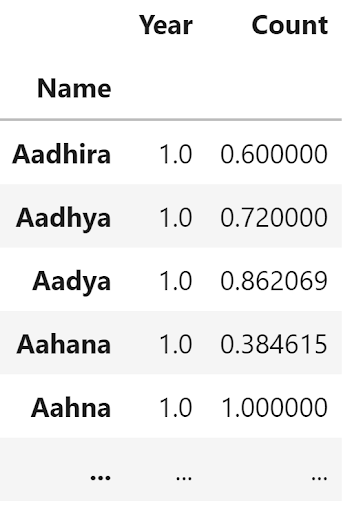
\includegraphics[width=0.5\textwidth]{4-agg1.png}
\end{center}
\end{minipage}
\begin{minipage}{0.5\textwidth}
Dropping Columns:
\begin{center}
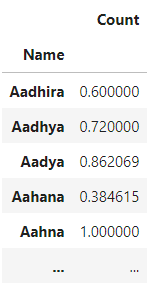
\includegraphics[width=0.4\textwidth]{4-agg2.png}
\end{center}
\end{minipage}
\end{notebox}

\textbf{Renaming Columns}

Use \mintinline{text}{.rename} (General Form: \mintinline{text}{df.rename(columns= \{<old colname1>: <new colname1>, ..., <old-colnameN>: <new-colnameN> \})}) to rename columns.
\begin{minted}{python}
rtp_table = female_babynames.groupby("Name")[["Count"]].agg(ratio_to_peak)
rtp_table = rtp_table.rename(columns = {"Count": "Count RTP"}) # change colname using a dict
\end{minted}

\begin{example}[]{Write a \mintinline{text}{groupby.agg} call that returns the total number of babies with the same name.
\tcbline 
As each entry records the name, year, and the count of babies born that year with the name, we should group by name and take the count column, then aggregate by the sum of the count in each year.
\begin{minted}{python}
ex1 = female_babynames.groupby("Name")[["Count"]].agg(sum)
\end{minted}
}
\end{example}

\begin{example}[]{Write a \mintinline{text}{grouby.agg} call that returns the total number of babies born per year.
\tcbline 
Again, each entry records name, year, and count of babies born that year. Therefore, it makes sense to group by year and aggregate by the total count for each entry in each year.
\begin{minted}{python}
ex2 = female_babynames.groupby("Year")[["Count"]].agg(sum)
\end{minted}
}
\end{example}

\begin{notebox}[Shorthand groupby methods]
Pandas has shorthand functions to use in place of \mintinline{text}{agg}, e.g. instead of \mintinline{text}{.agg(sum)}, you can use \mintinline{text}{.sum()}.

For more reference, check the Pandas reference \href{https://pandas.pydata.org/docs/reference/api/pandas.core.groupby.GroupBy.sum.html}{\color{blue}here}.
\end{notebox}

\subsubsection{Quick Look at EDA}
If we plot the table, we get the following graph of babies born per year. Does this say anything about the birth rate?

\begin{figure}[ht]
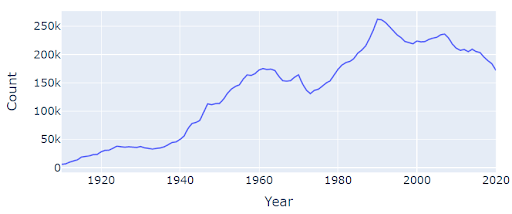
\includegraphics[width=0.75\textwidth]{4-birthrate}\centering\caption{Graph of the dataframe as the birthrate.}
\end{figure}
However, the birthrate in 2020 is closer to 400k instead of 200k. What went wrong? Upon checking the data, we find some biases and issues. We only used female babies, not all babies are registered for social security, and the database does not have some of the more uncommon names (e.g. ones that appear fewer than 5 times per year). Therefore, it's important to look at the data and understand it as opposed to using it blindly.

\begin{example}[]{Why does the following table claim that Woodrow Wilson won the presidency in 2020? The function call is as follows:
\begin{minted}{python}
elections.groupby("Party").agg(max).head(10)
\end{minted}
}
\tcbline
This groups by party and aggregates the max value. However, it aggregates the max value for each column. The max year would be the most recent - 2020, and Woodrow Wilson's name is last alphabetically, so it is last in the party, leading to this false result.

\textbf{Follow up:} Write code that returns the best percent result in each party.
\tcbline 
Start by sorting the percent results. Then, we want to group by the party and return the first value in the percent results table.
\begin{minted}{python}
top_results = elections.sort_values("%", ascending=False)
top_results_party = top_results.groupby("Party").agg(lambda x: x.iloc[0]) # gets the first row of each party group
\end{minted}
\end{example}

\begin{notebox}[]
In Pandas, there are multiple ways to get the same result - each way has tradeoffs in terms of readability, performance, memory, and complexity. it may take a while to understand these tradeoffs, so a general method is to change appraoches if one becomes too convoluted.
\end{notebox}

\subsubsection{Other groupby Features}
So far, we've only used \mintinline{text}{.agg}, which organizes all rows of the same group into a subframe for that group, then creates a new dataframe with each group as a row and combines the values with the given function.

\begin{minted}{python}
df.groupby("year").agg(sum) # each year split into a subframe for that year, new df with each year as a row, the value output is the sum of all the subframe values
\end{minted}

However, if you just call \mintinline{text}{groupby}, then you end up with a \mintinline{text}{DataFrameGroupBy} object, which can be combined with many functions (other than \mintinline{text}{.agg}) to generate DataFrames. Some choices include the following:
\begin{itemize}
\item \mintinline{text}{.agg}: creates a new dataframe with one aggregated row per subframe.
\item \mintinline{text}{.max}: creates a new dataframe aggregated with the max function.
\item \mintinline{text}{.size}: creates a new series with the size of each subframe.
\item \mintinline{text}{.filter}: creates a copy of the original dataframe, but only keeps the rows that satisfy the filter function.
\end{itemize}
More methods can be found on the Pandas reference \href{https://pandas.pydata.org/docs/reference/groupby.html}{\color{blue}here}.
(add some tikz/figures/tables)

\subsection{Pivot Tables}
If we want to group by multiple columns (e.g. using the babynames table, group by year and sex), we can group by both columns of interest. This creates a multi-indexed dataframe.

Another approach (from Data 8) is to pivot instead using the \mintinline{text}{pivot_table} function.

(General Use: \mintinline{text}{df.pivot_table(index=<col1>, columns=<col2>, values=[<val-cols>], aggfunc=<group-op>)})

\begin{minted}{python}
babynames.groupby(["Year", "Sex"]).agg(sum).head(6) # group with multiple cols
babynames.pivot_table(index="Year", columns="Sex", values=["Count"], aggfunc=np.sum) # pivot approach: sum up the count for each year/sex combination
\end{minted}

\begin{minipage}{0.5\textwidth}
\begin{center}
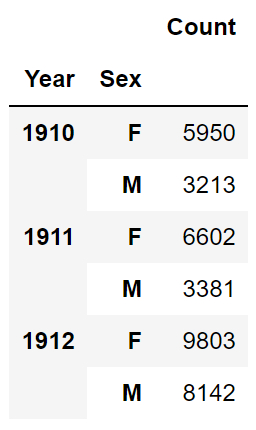
\includegraphics[width=0.4\textwidth]{4-multigroup.png}
\end{center}
\end{minipage}
\begin{minipage}{0.5\textwidth}
\begin{center}
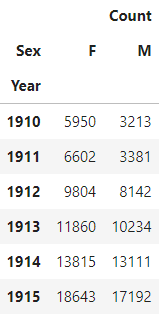
\includegraphics[width=0.4\textwidth]{4-pivot.png}
\end{center}
\end{minipage}

You can also have pivot tables with multiple columns.
\begin{minted}{python}
babynames.pivot_table(index=["Year", "Name"], columns="Sex", values=["Count"], aggfunc=np.max)
\end{minted}
\begin{figure}[ht]
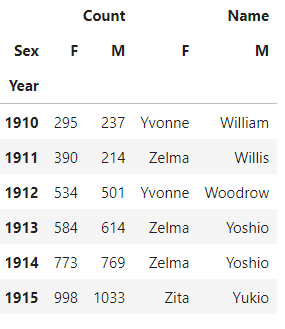
\includegraphics[width=0.35\textwidth]{4-multipivot.png}\centering\caption{Pivot with multiple columns. Adds another pivoted column like the column present in the previous pivot table.}
\end{figure}

\subsection{Joining Tables: An Overview}
Suppose we want to know the popularity of presidential names among male names. To do this, we need to join tables using \mintinline{text}{pd.merge}.

(General Usage: \mintinline{text}{df.merge(left=<table1>, right=<table2>, left_on=<col1>, right_on=<col2>)})

\begin{minted}{python}
# creating tables - table containing baby names and candidate names
male_2020_babynames = babynames.query('Sex == "M" and Year == 2020')
elections["First Name"] = elections["Candidate"].str.split().str[0]
merged = pd.merge(left = elections, right = male_2020_babynames, left_on = "First Name", right_on = "Name") # merge the two tables, left_on/right_on is the common column
\end{minted}


